\chapter{Specifikacija programske potpore}
		
	\section{Funkcionalni zahtjevi}
			
			\noindent \textbf{Dionici:}
			
			\begin{packed_enum}
				
				\item Regitrirani korisnik
					\begin{packed_enum}
						\item Klijent
						\item Administrator
					\end{packed_enum}
				\item Neregistrirani (anonimni) korisnik
				\item Razvojni tim
				\item Gradski ured
				
			\end{packed_enum}
			
			\noindent \textbf{Aktori i njihovi funkcionalni zahtjevi:}
			
			
			\begin{packed_enum}
				\item  \underbar{Klijent (inicijator) može:}
				
				\begin{packed_enum}
					
					\item Prijaviti se u sustav koristeći svoj email i lozinku
					\item Uređivati osobne podatke
					\item Poslati prijavu u sustav
					\begin{packed_item}
					\item Unijeti naziv za prijavu, opis prijave, geografske koordinate, te opcionalno fotografiju
					\item Odabrati koordinate preko karte ili unijeti najbližu adresu
					\item Povezati svoju prijavu na postojeću (ako takva postoji)
					\end{packed_item}
					\item Pregledati prijave i podatke vezane za njih
					\begin{packed_item}
					\item Odabrati aktivnu prijavu na karti
					\item Pregledati povijest svojih prijava
					\item Filtrirati pregled prijava po lokaciji i temi
					\end{packed_item}
					\item Registrirati novi gradski ured
					\item Zatražiti ulazak za participaciju u određeni gradski ured
					\item Mijenjati podatke aktivne prijave
				\end{packed_enum}
				
				\pagebreak
			
				\item  \underbar{Administrator (inicijator) može:}
				
				\begin{packed_enum}
					
					\item Pregledati popis svih prijava ikad napravljenih u sustavu
					\begin{packed_item}
					\item Uređivati podatke prijava
					\item Brisati prijave
					\end{packed_item}
					\item Pregledati i uklanjati registrirane profile po potrebi
					\item Odobravati kreaciju novih gradskih ureda
				\end{packed_enum}
				
				\item \underbar{Gradski ured (inicijator) može:}
				
				\begin{packed_enum}
					
					\item Pregledati popis aktivnih zaprimljenih prijava
					\begin{packed_item} 
					\item Prihvatiti (ili odbiti) određenu prijavu
					\item Spojiti nepovezane prijave
					\item Promijeniti status prihvaćene prijave ovisno o uspješnosti odrađene te iste prijave
					\end{packed_item}
					\item Prihvatiti (ili odbiti) zahtjev korisnika za ulazak u taj ured
					\item Poslati izvješće o odrađenoj prijavi na E-mail klijent
				\end{packed_enum}
				
				\item  \underbar{Neregistrirani korisnik (incijator) može:}
				
				\begin{packed_enum}
					\item Registrirati se u sustav koristeći ime, prezime, mail, username i lozinku
					\item Poslati prijavu u sustav
					\begin{packed_item}
					\item Unijeti naziv za prijavu, opis prijave, geografske koordinate, te opcionalno fotografiju
					\item Odabrati koordinate preko karte ili unijeti najbližu adresu
					\item Povezati svoju prijavu na postojeću (ako takva postoji)
					\item Zaprimiti jedistveni ID za podnesenu prijavu
					\end{packed_item}

				\end{packed_enum}
				
				\item  \underbar{Baza podataka (sudionik) može:}
				
				\begin{packed_enum}
				\item Pohraniti sve podatke o korisnicima i njihovim ovlastima
				\item Pohraniti svaku prijavu sa koreliranim podacima za istu	
				\end{packed_enum}
			\end{packed_enum}
			\eject 
			
			
				
			\subsection{Obrasci uporabe}
				
				\subsubsection{Opis obrazaca uporabe}
					

					\noindent \underbar{\textbf{UC01 - Registracija korisnika u sustav}}
					\begin{packed_item}
	
						\item \textbf{Glavni sudionik: }Neregistrirani korisnik
						\item  \textbf{Cilj:} Stvoriti korisnički račun
						\item  \textbf{Sudionici:} Baza podataka
						\item  \textbf{Preduvjet:} -
						\item  \textbf{Opis osnovnog tijeka:}
						
						\item[] \begin{packed_enum}
	
							\item Klijent bira opciju "registracija" na sučelju web aplikacicje
							\item Klijent unosi tažene podatke
							\item Korisnik je upisan u bazu podataka
						\end{packed_enum}
						
						\item  \textbf{Opis mogućih odstupanja:}
						
						\item[] \begin{packed_item}
	
							\item[2.a] Klijent unosi neispravni/postojeći username ili email
							\item[] \begin{packed_enum}
								
								\item Sustav obavještava korisnika o problemu i briše mu unesena polja
								
								\item Korisnik mijenja podatke u ispravne i registracija uspješno se privede kraju
								
							\end{packed_enum}
							
						\end{packed_item}
					\end{packed_item}
					
					\noindent \underbar{\textbf{UC02 - Unos nove prijave u sustav}}
					\begin{packed_item}
	
						\item \textbf{Glavni sudionik: }Korisnik
						\item  \textbf{Cilj:} Podnijeti novu prijavu
						\item  \textbf{Sudionici:} Baza podataka
						\item  \textbf{Preduvjet:} -
						\item  \textbf{Opis osnovnog tijeka:}
						
						\item[] \begin{packed_enum}
	
							\item Korisnik upisuje tražene podatke pri unosu prijave 
							\item Sustav javlja ako postoji vremenski bliska prijava na toj lokaciji
							\item Korisnik može povezati svoju prijavu na postojeću (ako takva postoji)
							\item Prijava se predaje i zapisuje u sustav
						\end{packed_enum}
						
						\item  \textbf{Opis mogućih odstupanja:}
						
						\item[] \begin{packed_item}
	
							\item[1.a] Korisnik nije naveo sve zahtijevane podatke
							\item[] \begin{packed_enum}
								
								\item Sustav obavještava korisnika o problemu i javlja mu da popuni tražena polja
								
							\end{packed_enum}
							
						\end{packed_item}
					\end{packed_item}
					
					\pagebreak
					
					\noindent \underbar{\textbf{UC03 - Pregled aktivnih prijava u sustavu}}
					\begin{packed_item}
	
						\item \textbf{Glavni sudionik: }Korisnik
						\item  \textbf{Cilj:} Pregled postojećih prijava
						\item  \textbf{Sudionici:} Baza podataka
						\item  \textbf{Preduvjet:} -
						\item  \textbf{Opis osnovnog tijeka:}
						
						\item[] \begin{packed_enum}
	
							\item Korisnik otvara pregled svih postojećih prijava
							\item Korisniku se nudi opcija filtriranja po temi i lokaciji
							\item Na sučelju se prikazuju filtritrane prijave
						\end{packed_enum}
					\end{packed_item}
					
					\noindent \underbar{\textbf{UC04 - Prijava u sustav}}
					\begin{packed_item}
	
						\item \textbf{Glavni sudionik: }Registrirani korisnik
						\item  \textbf{Cilj:} Prijaviti se svojim profilom u sustav
						\item  \textbf{Sudionici:} Baza podataka
						\item  \textbf{Preduvjet:} Registracija
						\item  \textbf{Opis osnovnog tijeka:}
						
						\item[] \begin{packed_enum}
	
							\item Korisnik upisuje korisničko ime i lozinku 
							\item Sustav javlja potvrdu ispravnosti unesinih podataka
							\item Korisniku se učitava njemu prilagođeno sučelje
						\end{packed_enum}
						
						\item  \textbf{Opis mogućih odstupanja:}
						
						\item[] \begin{packed_item}
	
							\item[1.a] Korisnik krivo unio korisničko ime/lozinku
							\item[] \begin{packed_enum}
								
								\item Sustav obavještava korisnika o problemu i javlja mu da ispravi tražena polja
								
								
							\end{packed_enum}
							
						\end{packed_item}
					\end{packed_item}
					
					\pagebreak
					
					\noindent \underbar{\textbf{UC05 - Uređivanje podataka prijave}}
					\begin{packed_item}
	
						\item \textbf{Glavni sudionik: }Administrator
						\item  \textbf{Cilj:} Korigirati podatke vezane za odabranu prijavu
						\item  \textbf{Sudionici:} Baza podataka
						\item  \textbf{Preduvjet:} Dodijeljena prava administratora
						\item  \textbf{Opis osnovnog tijeka:}
						
						\item[] \begin{packed_enum}
	
							\item Prikazuju se sve prijave
							\item Administrator može filtrirati prijave
							\item Administrator izmjenjuje podatke prijave
							\item Izmjenjena prijava se sprema u bazu podataka
						\end{packed_enum}
					\end{packed_item}
					
					\noindent \underbar{\textbf{UC06 - Brisanje prijave}}
					\begin{packed_item}
	
						\item \textbf{Glavni sudionik: }Administrator
						\item  \textbf{Cilj:} Obrisati određenu prijavu iz baze podataka
						\item  \textbf{Sudionici:} Baza podataka
						\item  \textbf{Preduvjet:} Dodijeljena prava administratora
						\item  \textbf{Opis osnovnog tijeka:}
						
						\item[] \begin{packed_enum}
	
							\item Administratoru se prikazuje pregled prijava  
							\item Administrator bira prijavu koju želi izbrisati
							\item Prijava se uklanja iz baze podataka i više nije vidljiva u aplikaciji
							
						\end{packed_enum}
					\end{packed_item}
					
					\noindent \underbar{\textbf{UC07 - Pregled podataka registriranih profila korisnika}}
					\begin{packed_item}
	
						\item \textbf{Glavni sudionik: }Administrator
						\item  \textbf{Cilj:} Uvid u profile registriranih korisnika i njihovih podataka
						\item  \textbf{Sudionici:} Baza podataka
						\item  \textbf{Preduvjet:} Dodijeljena prava administratora
						\item  \textbf{Opis osnovnog tijeka:}
						
						\item[] \begin{packed_enum}
	
							\item Korisnik bira opciju za pregled svih profila
							\item Otvara mu se lista svih registriranih profila zajedno sa njihovim osobnim podacima
							
						\end{packed_enum}
					\end{packed_item}
					
					\pagebreak
					
					\noindent \underbar{\textbf{UC08 - Pregled liste osobnih podataka vlastitog profila}}
					\begin{packed_item}
	
						\item \textbf{Glavni sudionik: }Klijent
						\item  \textbf{Cilj:} Pregledati osobne podatke svog profila
						\item  \textbf{Sudionici:} Baza podataka
						\item  \textbf{Preduvjet:} Registracija
						\item  \textbf{Opis osnovnog tijeka:}
						
						\item[] \begin{packed_enum}
	
							\item Korisnik ulazi u opis svog profila
							\item Sustav mu prikaže username, e-mail i lozinku
							
						\end{packed_enum}
					\end{packed_item}
					
					\noindent \underbar{\textbf{UC09 - Odjava iz sustava}}
					\begin{packed_item}
	
						\item \textbf{Glavni sudionik: }Registrirani korisnik
						\item  \textbf{Cilj:} Odjaviti se iz sustava
						\item  \textbf{Sudionici:} Baza podataka
						\item  \textbf{Preduvjet:} Aktivna prijava
						\item  \textbf{Opis osnovnog tijeka:}
						
						\item[] \begin{packed_enum}
	
							\item Korisnik bira opciju odjava 
							\item Sustav ga vraća na početnu stranicu web aplikacije
						\end{packed_enum}
					\end{packed_item}
					
					\noindent \underbar{\textbf{UC10 - Brisanje korisničkog računa}}
					\begin{packed_item}
	
						\item \textbf{Glavni sudionik: }Administrator
						\item  \textbf{Cilj:} Obrisati određeni profil
						\item  \textbf{Sudionici:} Baza podataka
						\item  \textbf{Preduvjet:} Dodijeljena prava administratora
						\item  \textbf{Opis osnovnog tijeka:}
						
						\item[] \begin{packed_enum}
	
							\item Administrator bira profil koji želi ukloniti
							\item Sustav ga za provjeru pita da potvrdi odluku
							\item Administrator potvrđuje i profil se uklanja iz baze podataka
						\end{packed_enum}
					\end{packed_item}
					
					\pagebreak
					
					\noindent \underbar{\textbf{UC11 - Pregledavanje povijesti svojih prijava}}
					\begin{packed_item}
	
						\item \textbf{Glavni sudionik: }Klijent
						\item  \textbf{Cilj:} Pregledati svu povijest privedenih prijava
						\item  \textbf{Sudionici:} Baza podataka
						\item  \textbf{Preduvjet:} Registracija
						\item  \textbf{Opis osnovnog tijeka:}
						
						\item[] \begin{packed_enum}
	
							\item Korisnik bira opciju za prikazivanje povijesti prijava 
							\item Sustav mu na sučelju prikazuje sve njegove prijave
							\item Korisnik dodatno može filtrirati iste po temi i lokaciji
						\end{packed_enum}
						
					\end{packed_item}
					
					\noindent \underbar{\textbf{UC12 - Pregledavanje profila gradskih ureda}}
					\begin{packed_item}
	
						\item \textbf{Glavni sudionik: }Administrator
						\item  \textbf{Cilj:} Pregledati popis svih postojećih gradskih ureda
						\item  \textbf{Sudionici:} Baza podataka
						\item  \textbf{Preduvjet:} Dodijeljena prava administratora
						\item  \textbf{Opis osnovnog tijeka:}
						
						\item[] \begin{packed_enum}
	
							\item Administrator odabire opciju za pregled svih gradskih ureda zapisanih u sustavu
							\item Sustav mu na sučelje prikazuje gradske urede zapisane u bazi podataka zajedno sa njihovim opisima
						\end{packed_enum}
					\end{packed_item}
					
					\noindent \underbar{\textbf{UC13 - Povezivanje na postojeću prijavu}}
					\begin{packed_item}
	
						\item \textbf{Glavni sudionik: }Korisnik
						\item  \textbf{Cilj:} Vezati se na vremenski blisku prijavu na istom području
						\item  \textbf{Sudionici:} Baza podataka
						\item  \textbf{Opis osnovnog tijeka:}
						
						\item[] \begin{packed_enum}
	
							\item Korisnik predaje prijavu
							\item Sustav mu javlja za vremenski blisku prijavu na toj lokaciji
							\item Korisnik bira hoće li se vezati na postojeću prijavu ili kreirati vlastitu
						\end{packed_enum}
					\end{packed_item}
					
					\pagebreak
					
					\noindent \underbar{\textbf{UC14 - Odabir aktivnih prijava sa karte}}
					\begin{packed_item}
	
						\item \textbf{Glavni sudionik: }Klijent
						\item  \textbf{Cilj:} Pogledati na karti neriješene prijave i detalje za iste
						\item  \textbf{Sudionici:} Baza podataka
						\item  \textbf{Preduvjet:} Postojanje aktivnih prijava
						\item  \textbf{Opis osnovnog tijeka:}
						
						\item[] \begin{packed_enum}
	
							\item Klijent na karti odabire opciju za uvid u aktivne prijave 
							\item Sustav mu sve lokacije aktivnih prijava prikazuje na karti
						\end{packed_enum}
						
						\item  \textbf{Opis mogućih odstupanja:}
						
						\item[] \begin{packed_item}
	
							\item[1.a] U sustavu nema aktivnih prijava
							\item[] \begin{packed_enum}
								
								\item Sustav korisnika izbacuje iz pregleda karte i javlja mu da nema aktivnih prijava	
							\end{packed_enum}
							
						\end{packed_item}
					\end{packed_item}
					
					\noindent \underbar{\textbf{UC15 - Mijenjanje sadržaja aktivne prijave}}
					\begin{packed_item}
	
						\item \textbf{Glavni sudionik: }Klijent
						\item  \textbf{Cilj:} Promijeniti sadržaj vlastite aktivne prijave
						\item  \textbf{Sudionici:} Baza podataka
						\item  \textbf{Preduvjet:} Postojanje aktivne prijave
						\item  \textbf{Opis osnovnog tijeka:}
						
						\item[] \begin{packed_enum}
	
							\item Klijent odabire svoju aktivnu prijavu koju želi izmjeniti
							\item Klijent mijenja atribut u prijavi
							\item Prijava s ažuriranim podakom se zapisuje u bazu podataka
						\end{packed_enum}
						
						\item  \textbf{Opis mogućih odstupanja:}
						
						\item[] \begin{packed_item}
	
							\item[1.a] U trenutku odabira prijave, prijava više nije aktivna
							\item[] \begin{packed_enum}
								
								\item Sustav korisniku javlja da prijava više nije aktivna	
								\item Korisnik je preusmjeren na početnu stranicu
							\end{packed_enum}
						\end{packed_item}
					\end{packed_item}
					
					\noindent \underbar{\textbf{UC16 - Pregled zaprimljenih prijava}}
					\begin{packed_item}
	
						\item \textbf{Glavni sudionik: }Gradski ured
						\item  \textbf{Cilj:} Pregledati sve zaprimljene prijave
						\item  \textbf{Sudionici:} Baza podataka
						\item  \textbf{Preduvjet:} Postojanje zaprimljenih prijava
						\item  \textbf{Opis osnovnog tijeka:}
						
						\item[] \begin{packed_enum}
	
							\item Gradski ured bira izabire pregled svih aktivnih prijava
							\item Sustav mu iz baze podataka omogući uvid u sve prijave namijenjene njemu
						\end{packed_enum}
						
						\item  \textbf{Opis mogućih odstupanja:}
						
						\item[] \begin{packed_item}
	
							\item[2.a] Nepostojanje prijava namijenjenih njemu
							\item[] \begin{packed_enum}
								
								\item Sustav mu javlja da trenutno nema aktivnih prijava	
							\end{packed_enum}
						\end{packed_item}
					\end{packed_item}
					
					\noindent \underbar{\textbf{UC17 - Prihvaćanje ili odbijanje zaprimljene prijave}}
					\begin{packed_item}
	
						\item \textbf{Glavni sudionik: }Gradski ured
						\item  \textbf{Cilj:} Privatiti ili odbiti prijavu iz pregleda prijava
						\item  \textbf{Sudionici:} Baza podataka, Gradski uredi
						\item  \textbf{Preduvjet:} -
						\item  \textbf{Opis osnovnog tijeka:}
						
						\item[] \begin{packed_enum}
	
							\item Gradski ured u pregledu svih prijava bira za pojedinu prijavu hoće li je prihvatiti ili odbiti
							\item U slučaju prihvaćanja prijave, ta se ista uklanja it popisa aktivnih drugim uredima za koje je bila namijenjena
						\end{packed_enum}
						
					\end{packed_item}
					
					\noindent \underbar{\textbf{UC18 - Promjena statusa određene prijave}}
					\begin{packed_item}
	
						\item \textbf{Glavni sudionik: }Gradski ured
						\item  \textbf{Cilj:} Promijeniti status prihvaćene prijave
						\item  \textbf{Sudionici:} Baza podataka
						\item  \textbf{Preduvjet:} Prihvat određene prijave
						\item  \textbf{Opis osnovnog tijeka:}
						
						\item[] \begin{packed_enum}
	
							\item Gradski ured za prihvaćaenu prijavu mijenja njen status ovisno je li uspješno odrađena ili ne
							\item Status se zapisuje u bazu podatka
							\item U slučaju neuspješno odrađene prijave, ta se ista vraća u popis aktivnih svim uredima za koje je i prije bila namijenjena
						\end{packed_enum}
						
					\end{packed_item}
					
					\noindent \underbar{\textbf{UC19 - Povezivanje nepovezanih prijava}}
					\begin{packed_item}
	
						\item \textbf{Glavni sudionik: }Gradski ured
						\item  \textbf{Cilj:} Spojiti više pojedinih prijava u jednu cjelinu
						\item  \textbf{Sudionici:} Baza podataka, Korisnik (inicjaitaor prijave)
						\item  \textbf{Preduvjet:} -
						\item  \textbf{Opis osnovnog tijeka:}
						
						\item[] \begin{packed_enum}
	
							\item Gradski ured iz pregleda prijava odabire prijave koje želi povezati
							\item Svaki prijavitelj čija je prijava povezana na druge sada to vidi u sustavu
						\end{packed_enum}
						
					\end{packed_item}
					
					\pagebreak
					
					\noindent \underbar{\textbf{UC20 - Prihvaćanje zahtjeva za ulazak registriranog korisnika u gradski ured}}
					\begin{packed_item}
	
						\item \textbf{Glavni sudionik: }Gradski ured
						\item  \textbf{Cilj:} Prihvatiti ili odbiti zahtjev kroisnika za ulazak u  gradski ured
						\item  \textbf{Sudionici:} Baza podataka, Korisnik (inicijator zahtjeva)
						\item  \textbf{Preduvjet:} Poslan zahtjev za ulazak u gradski ured
						\item  \textbf{Opis osnovnog tijeka:}
						
						\item[] \begin{packed_enum}
	
							\item Gradski ured gleda poslane zahtjeve vezane za učlanjenje korisnika u taj određeni ured
							\item U slučaju da zahtjevi postoje gradski ured bira hoće li prihvatiti novog člana ili ne

						\end{packed_enum}
						
						\item  \textbf{Opis mogućih odstupanja:}
						
						\item[] \begin{packed_item}
	
							\item[1.a] Nepostojanje aktivnih zahtjeva za ulazak u ured
							\item[] \begin{packed_enum}
								
								\item Sustav javlja da trenutno nema poslanih zahtjeva	
							\end{packed_enum}
						\end{packed_item}
						
					\end{packed_item}
					
					\noindent \underbar{\textbf{UC21 - Slanje zahtjeva za ulazak u gradski ured}}
					\begin{packed_item}
	
						\item \textbf{Glavni sudionik: }Registrirani korisnik
						\item  \textbf{Cilj:} Poslati određenom gradskom uredu zahtjev za ulaz u isti
						\item  \textbf{Sudionici:} Baza podataka, Gradski ured
						\item  \textbf{Preduvjet:} -
						\item  \textbf{Opis osnovnog tijeka:}
						
						\item[] \begin{packed_enum}
	
							\item Korisnik odabire u tražilici određeni gradski ured
							\item Pri pronalasku traženog ureda korisnik šalje zahtjev za ulaz u isti

						\end{packed_enum}
						
					\end{packed_item}
					
					\noindent \underbar{\textbf{UC22 - Registracija novog gradskog ureda}}
					\begin{packed_item}
	
						\item \textbf{Glavni sudionik: }Registrirani korisnik
						\item  \textbf{Cilj:} Kreirati novi gradski ured
						\item  \textbf{Sudionici:} Baza podataka, Administrator
						\item  \textbf{Preduvjet:} -
						\item  \textbf{Opis osnovnog tijeka:}
						
						\item[] \begin{packed_enum}
	
							\item Korisnik odabire opciju kreiraj gradski ured
							\item Pri kreiranju novog gradskog ureda unosi podatke za isti
							\item Na temelju podataka administrator i baza podataka prihvaćaju ili odbijaju zahtjev za kreiranjem ureda

						\end{packed_enum}
						
					\end{packed_item}
					
					\pagebreak
					
					\noindent \underbar{\textbf{UC23 - Uređivanje osobnih podataka}}
					\begin{packed_item}
	
						\item \textbf{Glavni sudionik: }Klijent
						\item  \textbf{Cilj:} Promijeniti osobne podatke u bazi podataka
						\item  \textbf{Sudionici:} Baza podataka
						\item  \textbf{Preduvjet:} -
						\item  \textbf{Opis osnovnog tijeka:}
						
						\item[] \begin{packed_enum}
	
							\item Korisnik bira opciju uređavanje osobnih podataka
							\item Mijenja podatak, te se novi zapisuje u bazu podataka

						\end{packed_enum}
						\item  \textbf{Opis mogućih odstupanja:}
						
						\item[] \begin{packed_item}
	
							\item[2.a] Unos neispravnog podatka
							\item[] \begin{packed_enum}
								
								\item Baza podatka mu dojavljuje o grešci i traži ga da promijeni unos	
								\item Korisnik odustaje od unosa ili prepravlja unos podataka
							\end{packed_enum}
						\end{packed_item}
						
					\end{packed_item}
					
					\noindent \underbar{\textbf{UC24- Praćanje prijave jedinstvenim ID-om}}
					\begin{packed_item}
	
						\item \textbf{Glavni sudionik: }Neregistrirani korisnik
						\item  \textbf{Cilj:} Pregledati svou prijavu unosom jedinstvenog broja
						\item  \textbf{Sudionici:} Baza podataka
						\item  \textbf{Preduvjet:} Postojanje jedinstvenog broja
						\item  \textbf{Opis osnovnog tijeka:}
						
						\item[] \begin{packed_enum}
	
							\item Neregistrirani korisnik u tražilicu unosi ID koji je dobio pri unosu prijave
							\item Sustav mu pokaže njegovu prijavu i status ako je unesen broj važeći
						\end{packed_enum}
						\item  \textbf{Opis mogućih odstupanja:}
						
						\item[] \begin{packed_item}
	
							\item[1.a] Unos neispravnog podatka
							\item[] \begin{packed_enum}
								
								\item Baza podatka mu dojavljuje o grešci i traži ga unese ispravan ID ili da odustane od prijave
								\item Korisnik bira opciju odustani ili opet unosi ID	
							\end{packed_enum}
						\end{packed_item}
						
					\end{packed_item}
					
					\noindent \underbar{\textbf{UC25- Slanje obavijesti vezane za odrađenu prijavu na E-mail klijent }}
					\begin{packed_item}
	
						\item \textbf{Glavni sudionik: }Gradski ured
						\item  \textbf{Cilj:} Isporučiti objavu vezanu za odrađenu prihvaćenu prijavu na E-mail klijenta
						\item  \textbf{Sudionici:} E-mail klijent
						\item  \textbf{Preduvjet:} -
						\item  \textbf{Opis osnovnog tijeka:}
						
						\item[] \begin{packed_enum}
	
							\item Gradski ured šalje prouku o prijavi na E-mail klijent 
							\item E-mail klijent prikazuje podnositelju prijave obavijest
						\end{packed_enum}
						
					\end{packed_item}
						
				
					
				\subsubsection{Dijagrami obrazaca uporabe}
					
					\begin{figure}[H]
			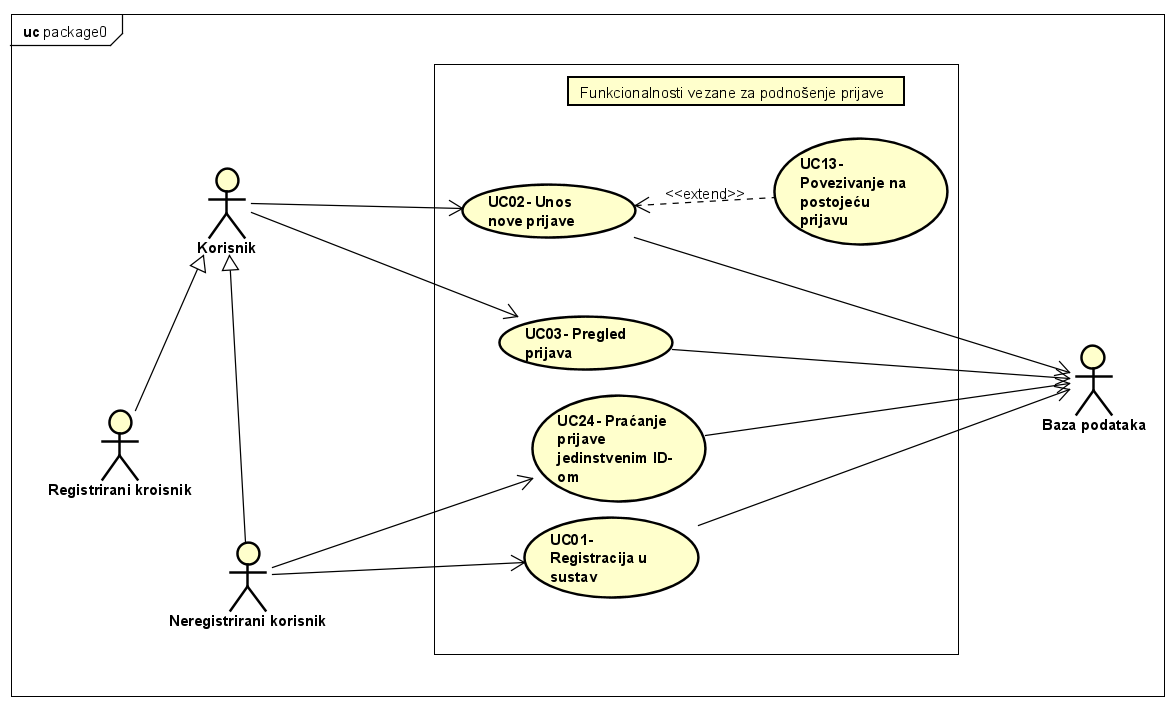
\includegraphics[scale=0.8]{slike/obrazac_podnosenjeprijave.PNG} %veličina slike u odnosu na originalnu datoteku i pozicija slike
			\centering
			\caption{Dijagram obrasca uporabe - Funkcionalnosti vezane za podnošenje prijave}
		\end{figure}
		
		
		\begin{figure}[H]
			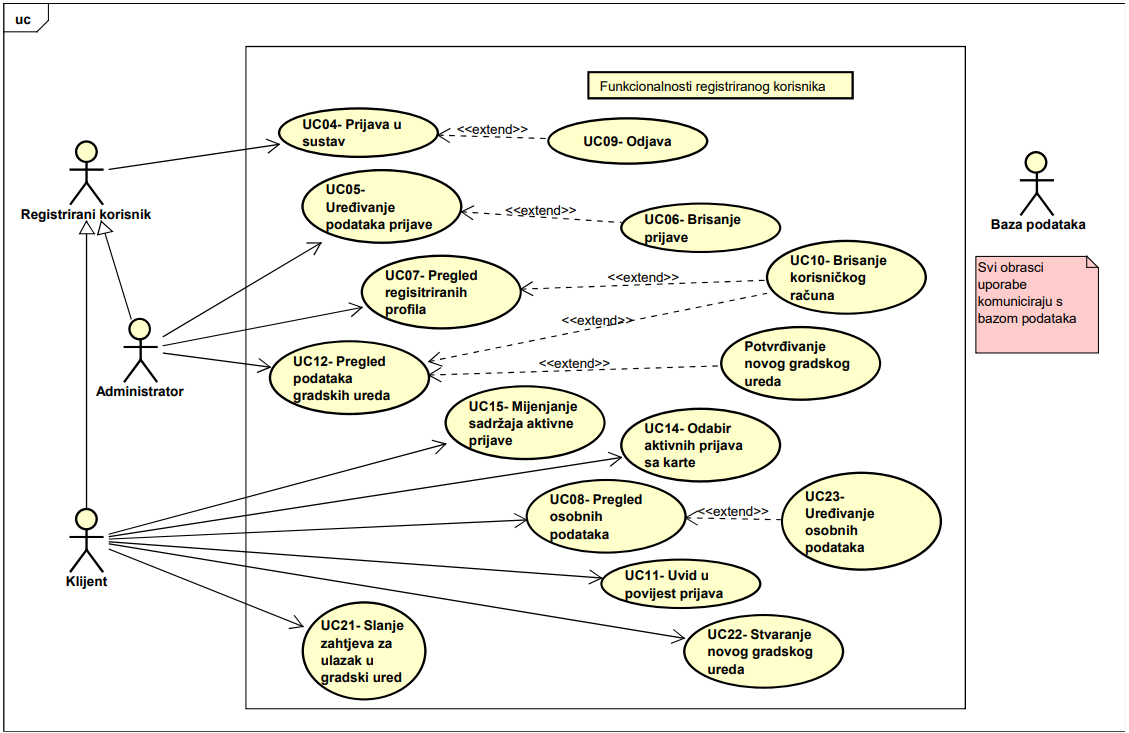
\includegraphics[scale=0.8]{slike/obrazac_registereduser.PNG} %veličina slike u odnosu na originalnu datoteku i pozicija slike
			\centering
			\caption{Dijagram obrasca uporabe - Funkcionalnosti registriranog korisnika (administrator i klijent)}
		\end{figure}		
				
				
				\begin{figure}[H]
			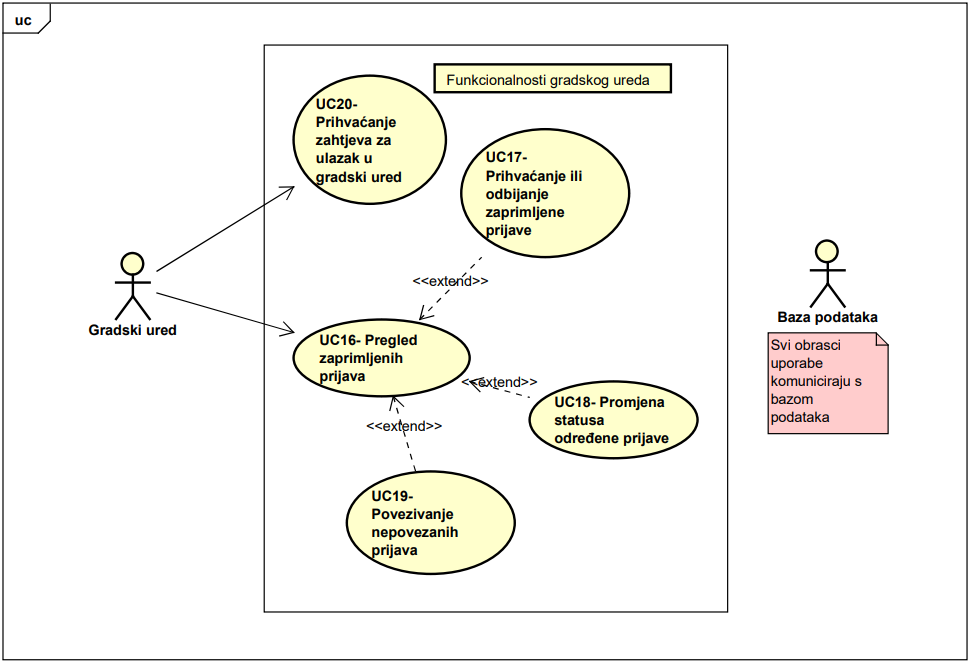
\includegraphics[scale=0.8]{slike/obrazac_gradski.PNG} %veličina slike u odnosu na originalnu datoteku i pozicija slike
			\centering
			\caption{Dijagram obrasca uporabe - Funkcionalnosti gradskog ureda}
		\end{figure}
			\subsection{Sekvencijski dijagrami}
				
				\textbf{\textit{dio 1. revizije}}\\
				
				
				\textit{Nacrtati sekvencijske dijagrame koji modeliraju najvažnije dijelove sustava (max. 4 dijagrama). Ukoliko postoji nedoumica oko odabira, razjasniti s asistentom. Uz svaki dijagram napisati detaljni opis dijagrama.}
				\\
				\\
				\textbf{TODO: ako treba prenijeti dokumentaciju u wiki pa nacrtati specificirane dijagrame obrazaca uporabe i sekvencijske}
				\\
				\\
				\textbf{Obrasci uporabe UC02, UC03, UC13, UC14 - unos nove prijave, pregled postojećih prijava, povezivanje na postojeću prijavu, uvid u aktivne prijave sa karte}\\
				Korisnik (prijavljeni ili anonimni) može podnijeti novu prijavu sustavu. Korisnik odabire opciju unosa nove prijave nakon čega poslužitelj vraća formu za upis podataka prijave. 
				Korisnik šalje prijavu te sustav provjerava unos korisnika i provjerava u postoje li vremenski i prostorno bliske aktivne prijave te ako postoje, vraća formu korisniku gdje se može spojiti na neku od bliskih prijava. 
				Korisnik šalje poslužitelju hoće li se i na koju povezati te poslužitelj sprema novu prijavu u bazu podataka. Korisnik također može poslati zahtjev za pregledom svih postojećih prijava uz opcionalne filtere po temi i lokaciji na što poslužitelj reagira dohvaćanjem tih podataka iz baze te slanjem istih korisniku. 
				Korisnik također može kliknuti na neku od aktivnih prijava na karti na što se poslužitelju šalje zahtjev na koji on reagira dohvaćanjem detalja te prijave iz baze podataka te odgovaranjem korisniku istima.
				
				
				\textbf{Obrazac uporabe UC01 - registracija korisnika u sustav}\\
				Neprijavljeni korisnik može poslati zahtjev za registracijom na što poslužitelj odgovara formom za registraciju. Kad korisnik pošalje podatke, poslužitelj ih validira te sprema u bazu podataka.

				\textbf{Obrazac uporabe UC05, UC06, UC07, UC10 - uređivanje podataka prijave, brisanje prijave, pregled korisnika, brisanje korisničkog računa, pregled gradskih ureda}\\
				Adminisistrator može poslati zahtjev poslužitelju za uređivanje podataka iz pojedine prijave na što poslužitelj zahtjeva podatke te prijave iz baze te ih u formi za uređivanje vraća administratoru. Nakon uređivanja administrator šalje nove podatke poslužitelju na što ih on sprema u bazu.
				Administrator također može poslati poslužitelju zahtjev za brisanjem prijave na što poslužitelj briše prijavu iz baze.
				Osim toga, administrator ima uvid i u sve registrirane korisnike kao liste koju na zahtjev poslužitelj zahtijeva iz baze te vraća administratoru.
				Osim korisnika, na isti način administrator može pregledati i gradske urede.

				\textbf{Obrazac uporabe UC04, UC08, UC11, UC15 - prijava korisnika u sustav, pregled osobnih podataka, pregled povijesti vlastitih prijava, mijenjanje sadržaja aktivne prijave}\\
				Registrirani korisnik može poslati zatjev za prijavom u sustav na što poslužitelj odgovara formom za prijavu. Kad korisnik prijavu pošalje, poslužitelj ju validira uz pomoć baze podataka te obaviještava korisnika o uspiješnosti prijave. Prijavljeni korisnik može poslati poslužitelju zahtjev za pregledom povijesti vlastitih prijava na što ih poslužitelj dohvaća iz baze podataka te ih vraća korisniku. Na isti način prijavljeni korisnik može pregledati osobne podatke.
				Ukoliko prijavljeni korisnik želi mijenati svoju aktivnu prijavu, može odabrati jednu iz liste aktivnih prijava na što se poslužitelju šalje zahtjev za uređivanjem iste. Poslužitelj tad dohvaća podatke te prijave iz baze podataka te korisniku šalje formu s podacima prijave. Korisnik tad uređuje podatke te ih šalje poslužitelju na što ih poslužitelj validira te sprema u bazu podataka.

				\eject
	
		\section{Ostali zahtjevi}
		
			\begin{packed_item}
			\item Sustav treba biti implementiran u obliku web aplikacije
			\item Aplikacija treba biti uvijek dostupna
			\item Aplikacije treba pružati usluge u stvarnom vremenu
			\item Učitavanje aplikacije ne smije trajati duže od 2 sekunde
			\item Pristup bazi podataka ne smije trajati duže od 2 sekunde
			\item Sustav treba biti organiziran u obliku MVC
			\item Sustav na poslužiteljskoj strani je napisan u programskom jeziku Java te radnom okviru Spring Boot
			\item Sustav na klijentskoj strani je implementiran programskim jezikom JavaScript te radnom okviru React.js
			\item Podaci se spremaju u bazu podataka koristeći JPA
			\item Arhitektura aplikacije mora biti u obliku klijent-poslužitelj
			\item Pri pristupu aplikaciji se koristi protokol HTTPS
			\item Aplikacije treba biti prilagođena i desktop uređajima kao i mobilnim uređajima
			\item Veza s bazom podataka mora biti kvalitetno zasti ˇ cena, brza i otporna na vanjske greške
			\item Pristup sustavu mora biti omogucen iz javne mreže pomoću HTTPS
			\end{packed_item}
			 